\chapter{Method and results}
\label{chap:method}

\section{Method}

The method relies on the model
\begin{equation}
  \label{eq:model}
  \frac{\mathrm{d}x}{\mathrm{d}t} = -\lambda x, \qquad x(0) = x_0,
\end{equation}
whose solution is $x(t) = x_0 e^{-\lambda t}$.

\section{Results}

Figure~\ref{fig:results} and Table~\ref{tab:results} present the results
obtained with model~\eqref{eq:model}.

\begin{figure}[htbp]
  \centering
  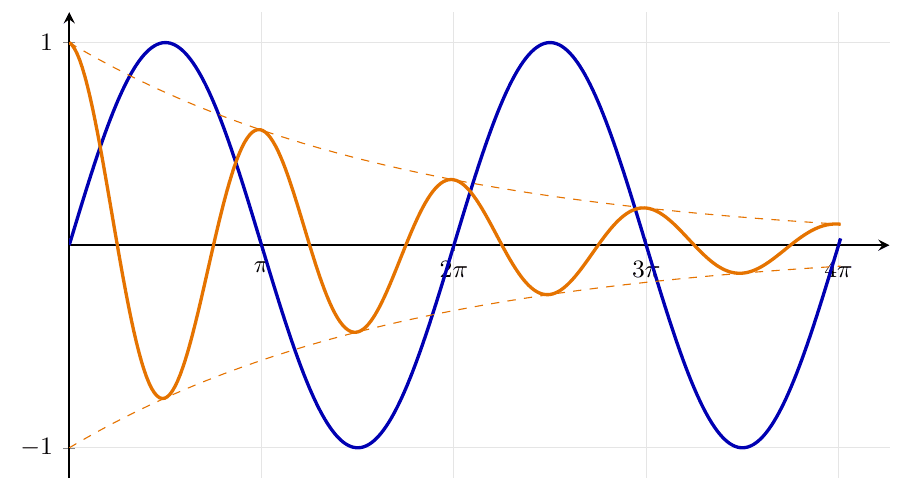
\includegraphics[width=0.75\linewidth]{images/curves.png}
  \caption{An image of the project: replace it with your results.}
  \label{fig:results}
\end{figure}

\begin{table}[htbp]
  \centering
  \caption{Estimated values of the parameter $\lambda$.}
  \label{tab:results}
  \begin{tabular}{lrr}
    \toprule
    Trial & $\lambda$ & Relative error (\%) \\
    \midrule
    1 & 0.182 & 1.1 \\
    2 & 0.179 & 0.6 \\
    3 & 0.185 & 2.8 \\
    \bottomrule
  \end{tabular}
\end{table}
